%%%%%%%%%%%%%%%%%%%%%%%%%%%%%%%%%%%%%%%%%%%%%%%%%%%%%%%%%%%%%
%% HEADER
%%%%%%%%%%%%%%%%%%%%%%%%%%%%%%%%%%%%%%%%%%%%%%%%%%%%%%%%%%%%%
\documentclass[a4paper,twoside,10pt]{report}



%% Language %%%%%%%%%%%%%%%%%%%%%%%%%%%%%%%%%%%%%%%%%%%%%%%%%
\usepackage[USenglish]{babel} %francais, polish, spanish, ...
\usepackage[T1]{fontenc}
\usepackage[ansinew]{inputenc}

\usepackage{lmodern} %Type1-font for non-english texts and characters


%% Packages for Graphics & Figures %%%%%%%%%%%%%%%%%%%%%%%%%%
\usepackage{graphicx} %%For loading graphic files

%% Math Packages %%%%%%%%%%%%%%%%%%%%%%%%%%%%%%%%%%%%%%%%%%%%
\usepackage{amsmath}
\usepackage{amsthm}
\usepackage{amsfonts}


%% Line Spacing %%%%%%%%%%%%%%%%%%%%%%%%%%%%%%%%%%%%%%%%%%%%%
%\usepackage{setspace}
%\singlespacing        %% 1-spacing (default)
%\onehalfspacing       %% 1,5-spacing
%\doublespacing        %% 2-spacing


%% Other Packages %%%%%%%%%%%%%%%%%%%%%%%%%%%%%%%%%%%%%%%%%%%
\usepackage{a4wide} %%Smaller margins = more text per page.
\usepackage{fancyhdr} %%Fancy headings
\usepackage{longtable} %%For tables, that exceed one page
\usepackage{hyperref}
\usepackage{booktabs}

%% LISTINGS %%%%%%%%%%%%%%%%%%%%%%%%%%%%%%%%%%%%%%%%%%%%%%%%%
\usepackage{listings}
\usepackage{color}
\definecolor{mygray}{rgb}{0.95,0.95,0.95}
\lstset{
  backgroundcolor=\color{mygray},
	numbers=left
}

%%%%%%%%%%%%%%%%%%%%%%%%%%%%%%%%%%%%%%%%%%%%%%%%%%%%%%%%%%%%%
%% Options / Modifications
%%%%%%%%%%%%%%%%%%%%%%%%%%%%%%%%%%%%%%%%%%%%%%%%%%%%%%%%%%%%%

%----------------------------------------------------------------------------------------
%	TITLE PAGE
%----------------------------------------------------------------------------------------

\newcommand*{\titleGM}{\begingroup % Create the command for including the title page in the document
\hbox{ % Horizontal box
\hspace*{0.2\textwidth} % Whitespace to the left of the title page
\rule{1pt}{\textheight} % Vertical line
\hspace*{0.05\textwidth} % Whitespace between the vertical line and title page text
\parbox[b]{0.75\textwidth}{ % Paragraph box which restricts text to less than the width of the page

{\noindent\Huge\bfseries Multimedia Report \\[0.5\baselineskip] Forum Application}\\[2\baselineskip] % Title
{\large \textit{Multimedia modelleren en programmeren}}\\[4\baselineskip] % Tagline or further description
{\Large \textsc{Joris Schelfaut}} % Author name

\vspace{0.5\textheight} % Whitespace between the title block and the publisher
	{\noindent Katholieke Universiteit Leuven}\\[\baselineskip] % Publisher and logo
}}
\endgroup}




%%%%%%%%%%%%%%%%%%%%%%%%%%%%%%%%%%%%%%%%%%%%%%%%%%%%%%%%%%%%%
%% DOCUMENT
%%%%%%%%%%%%%%%%%%%%%%%%%%%%%%%%%%%%%%%%%%%%%%%%%%%%%%%%%%%%%
\begin{document}

\pagestyle{empty} %No headings for the first pages.


\titleGM


\tableofcontents %Table of contents
\cleardoublepage %The first chapter should start on an odd page.

\pagestyle{plain} %Now display headings: headings / fancy / ...



%% Chapters %%%%%%%%%%%%%%%%%%%%%%%%%%%%%%%%%%%%%%%%%%%%%%%%%

% INTRODUCTION
\chapter{Introduction}

\section{About the course}

The course \emph{Multimedia: modelleren \& pogrammeren} is given by prof. E. Duval at KULeuven. The objective of this course to create a mobile application using different technologies, namely \texttt{iOS}, \texttt{Android} and \texttt{HTML5}, to eventually gain insight in the advantages and disadvantages of each technology.

The technologies that will be discussed on this blog are \texttt{iOS} and \texttt{Android}. All code for this project is open source and can be found on and downloaded from Github\footnote{\url{https://github.com/mumedev}}. The progress of the development is communicated through a blog\footnote{\url{http://mumedev.wordpress.com/}}.


\section{About the application}

The application is an online forum where the main question of each tread is directed at one expert or a group of experts. Each member can enlist him/herself as an expert in certain areas and will get notified when a question is posted, related to his/her domain of expertise.

%Badges can be obtained (providing useful comments for a number of problems), and certificates (having an actual degree in a certain area)
%if specific for KULeuven --> credits obtained for certain courses ~ expertise

Although similar websites already exist, e.g. \emph{Stackoverflow}\footnote{\url{http://stackoverflow.com/}} and \emph{Yahoo! Answers}\footnote{\url{http://answers.yahoo.com/}}, one idea would be to direct the application rather at students than at the general public. The idea arose when looking at the rather limited use of the fora on \emph{Toledo}\footnote{\url{https://toledo.kuleuven.be}}.


\section{Structure of this text}

The next chapter looks at the idea behind the application in more detail. We use tools such as user stories, story boards, use case diagrams, and screen transition diagrams to get an understanding of the application from a user's perspective. From these functional requirements, a number of general requirements for the software can be derived.

These requirements serve as the input for chapters \ref{chapter:architecture} and \ref{chapter:implementation}. In these chapter we will determine how the architecture of the application is constructed on three levels: a global scope, the data itself, and each app individually.

Chapter \ref{chapter:comparison} looks at different aspects of each mobile technology and tries to compare them.

Finally chapter \ref{chapter:conclusion} looks back at the project, points presented in the discussion, and the course as a whole.



% REQUIREMENT ANALYSIS
\chapter{Requirement analysis}\label{chapter:requirement_analysis}

\section{User story and storyboard}\label{section:story}

The use of the application can be illustrated by the following  user story. Figure \ref{figure:storyboard} depicts the same story line.

\begin{figure}
	
\includegraphics[width=200px]{img/filename}
	\caption{Story board depicting a potential scenario of use.}
	\label{figure:storyboard}
\end{figure}


%%%%%%%%%% USER STORY
\textit{Jake is a student at the department of computer science at KULeuven. For his project of Multimedia he has to develop an Android application. Unfortunately he has encountered a particular problem as he was working on the application. He decides to look for some help.}

\textit{He starts the application and enters his question. He also attaches a number of specialities as tags to his post. Users that are listed as specialists in these technologies are then notified and can start working on a solution.}

\textit{Several solutions are proposed. Jake finds one that works and is able to continue with his work.}


% tag system ---> hierarchical (but more specific tags may have multiple parents)

% open (still open for discussion) and closed questions
% public (visible for everyone) / private
% open forum (everyone can participate), closed forum

% the recipient of a question, can suggest other question recipients, or delegate the question

% chatbox available, but can be turned off, or made available for groups of people
% (if necessary only during selected periods of time, e.g. personalized help)
% tutors can get a licence to teach, private students can pay money for private lessons
% (in contrast to public lessons / questions)

% !!! "interests" :
%	person 1 :  I would like to learn skill X
%	person 2 : I would like to learn skill Y
%	person 3 : I am good at skill X
%	person 4 : I would like to help people with skill Y
%		SUGGESTION system :
%		person 1 and person 4 are matched
%		person 2 and person 3 can be matched as well... (e.g. to person 3: person 2 would like to learn a skill you are good at, care to help him/her?) How did you started learning this skill? ...


\section{Use case diagram}\label{section:usecase}

The use case diagram for the application is shown in  figure \ref{figure:use_case_diagram}. Each use case is elaborated in tables \ref{table:use_case1}, \ref{table:use_case2} and \ref{table:use_case3}.

\begin{figure}
	\begin{center}
		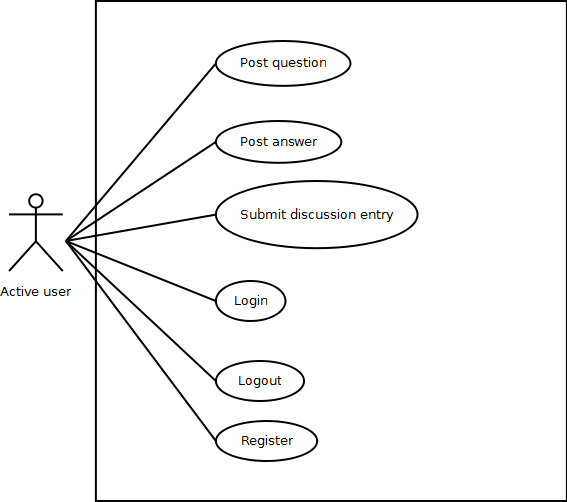
\includegraphics[width=200px]{img/use_case_diagram}
	\end{center}
	\caption{The use case diagram showing the functionality in the system from a user's perspective.}
	\label{figure:use_case_diagram}
\end{figure}


\begin{table}[h]
\caption{Use case 1 \textit{Post question}}
\begin{center}
	\begin{tabular}{ l p{300px} }
		\hline
		\textbf{Primary actor:}	& Active user \\

		\textbf{Preconditions:}	& User is logged in; \\

		\textbf{Basic flow:}	& (1) The question form is loaded. \\
													& (2) The user enters his question. \\
													& (3) The user selects recipients, including specific people and groups. \\
													& (4) The user submits the form data. \\
													& (5) The systems shows a confirmation message. \\

		\hline
	\end{tabular}
\end{center}
\label{table:use_case1}
\end{table}


\begin{table}[h]
\caption{Use case 2 \textit{Post answer}}
\begin{center}
	\begin{tabular}{ l p{300px} }
		\hline
		\textbf{Primary actor:}	& Active user \\

		\textbf{Preconditions:}	& User is logged in; \\
														& The user has selected a question to answer. \\
														& User is allowed to participate in the discussion. \\

		\textbf{Basic flow:}	& (1) The user selects an option to answer the question. \\
													& (2) The user enters his/her answer. \\
													& (3) The user submits the answer. \\
													& (4) The systems shows a confirmation message. \\

		\hline
	\end{tabular}
\end{center}
\label{table:use_case2}
\end{table}



\begin{table}[h]
\caption{Use case 3 \textit{Take part in discussion.}}
\begin{center}
	\begin{tabular}{ l p{300px} }
		\hline
		\textbf{Primary actor:}	& Active user \\

		\textbf{Preconditions:}	& The user is logged in; \\
														& The user has found a question he/she would like to provide further comments on; \\
														& The user is allowed to participate in the discussion.\\

		\textbf{Basic flow:}	& (1) The user selects an option to create a discussion entry. \\
													&	(2) The user types in the discussion entry.	\\
													& (3) The user submits the entry. \\
													& (4) The entry is added to the discussion. \\

		\hline
	\end{tabular}
\end{center}
\label{table:use_case3}
\end{table}



\section{Screen transition diagram}\label{section:screen_transitions}


\begin{figure}
	\begin{center}
		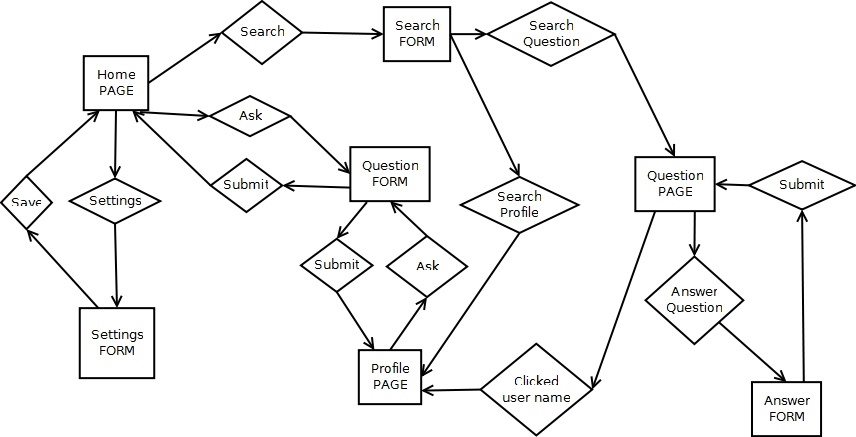
\includegraphics[width=400px]{img/screen_transition_diagram}
	\end{center}
	\caption{The transitions between the screens.}
	\label{figure:screen_transition_diagram}
\end{figure}

% ARCHITECTURE
\chapter{Architecture}\label{chapter:architecture}

% General architecture of the application
% central server with API and three mobile apps
% MVC REST API to mobile App
% MVC in the App's internal structure

%First we will discuss how the different components of the application's architecture are combined and communicate. Next we will give an overview of the how the data is structured. Finally we will look at each app in more detail.

% Architectural paradigms
%	Data organization and mobile computing
%
% heterogeneity also apparent in mobile apps themselves
%		(software : html5 vs android vs ios)
%		(performance : native vs web)
%		(hardware : e.g. android has to deal with different screen sizes)

% mobile computing
% Stefan Ternier proposes \cite{ternier:2012}

\section{Architectural challenges}

Before discussing the end result, we will try to give an overview of some of the challenges that need to be addressed when designing mobile applications. One of the central questions when building any application is how to organize information. Trade-offs in the design of data organization go beyond the level of the data itself. For example the physical location of data, i.e., whether data is kept locally or stored remotely. Availability, fault-tolerance and Quality of service (Qos), which covers reliability, security and performance, are other aspects that can be taken into account\cite{}.

To support interactions between users on different devices, some data will be sent over the network. Several communication paradigms exist, such as direct or indirect communication. The important difference here is that in the second case an additional layer of indirection exists, decoupling the producers and consumers of information streams\cite{coulouris:2012}. These communicating entities can also take on different roles, from a \emph{client-server} approach were clients are consumers and servers are producers, to a \emph{peer-to-peer} (P2P) architecture where conceptually only one type of role exists\cite{coulouris:2012}.

In a distributed environment software engineers may have to deal with a degree of heterogeneity both in software and hardware. As a result layers of transparency can be introduced to reduce complexity of the underlying structures.

Another challenge of the application that we are building is inherent to \emph{mobile computing}. Coulouris et al. define mobile computing as "the performance of computing tasks while the user is on the move, or visiting places other than their usual environment"\cite{coulouris:2012}. This poses a difficulty, as the quality of the connection may fluctuate, devices may be disconnected and reconnected as the user moves, or temporary go offline for an undefined period of time\cite{coulouris:2012}. Although this is an important aspect, it is not a major concern of the application as changes in the data may take several minutes to hours or days to take place. However, when creating data, it might be a good idea to give an option to store local drafts; for example when the connection is lost.


\section{Architecture design}

The roles of the communicating entities correspond to the client-server paradigm. The choice for this architecture is to provide a single point to access stored data. Storing all data locally and exchanging updates is possible, but would be a lot more complicated. Based on the characteristics of peer-to-peer systems, replication, CPU usage, and network traffic, introduce significant constraints on the mobile device's performance. Bandwidth, local storage and CPU are all much more limited than in home computers. In addition, due to their mobile nature, the physical layout of the network may change constantly. As a result, a client-server approach seems the logical choice. The global architecture is shown in figure \ref{figure:architecture:global}.

\begin{figure}
	
	\begin{center}
		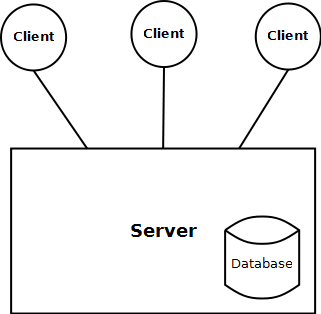
\includegraphics[width=200px]{img/architecture_global}
		\caption{The global architecture of the application.}
		\label{figure:architecture:global}
	\end{center}

\end{figure}

To allow access to the database, each application can talk to a public interface. For example, in listing \ref{listing:dbaccess} is shown how one could use \texttt{PHP} scripts to access the database, using URLs to pass arguments. This kind of approach is 

%% LISTING
%\lstinputlisting[language=PHP, caption={Example of a \texttt{PHP} script to insert data into the database (simplification).}, label={listing:dbaccess}]{code/dbaccess.php}

In this case, REST (Representational State Transfer) was used to implement this point of public access. The REST approach uses \texttt{HTTP} operations GET, PUT, DELETE and POST to manipulate resources represented in XML\cite{coulouris:2012}. The API shields the underlying data structures from the clients, organizes the application's data model into resources and can be accessed through a standardized protocol.

The REST API used here, consists out of a series of methods, as listed in table \ref{table:rest_api}. Five resources are provided: \emph{answer}, \emph{authentication}, \emph{question}, \emph{skill}, and \emph{user}.



\begin{table}
	\caption{REST API}\label{table:rest_api}
	
	\begin{center}
		\begin{tabular}{p{70px} | p{70px} | p{210px}}
				\hline
				\hline
				\textbf{Resource} 		& \textbf{Method}					&	\textbf{Description} 	\\
				\hline
				\hline
				\texttt{ANSWER}				& 												&	\\
				\hline
															& \emph{create}						& Create a new answer. \\
															& \emph{get\_question}		& Get the question this answer was posted on. \\
															%& \emph{search}						& Search an answer.	\\
				\hline
				\texttt{AUTHENTICATION}		& 												&	\\
				\hline
															& \emph{endsession}				& Create a new answer. \\
															& \emph{startsession}			& Get the question this answer was posted on. \\
				\hline
				\texttt{QUESTION}			& 												& \\
				\hline
															& \emph{create}						& Post a new question. \\
															& \emph{get\_answers}			& Get the answers for a question. \\
															& \emph{get\_info}				& Get information on a question. \\
															& \emph{get\_skills}			& Get the skills related to this question. \\
															& \emph{remove}						& Delete a question. \\
															%& \emph{search}						& Search questions, given a number of search parameters. \\
				\hline
				\texttt{SKILL}				& 												& \\
				\hline
															& \emph{create}						& Create a new skill and add it to the database. \\
															& \emph{get\_questions}		& Get questions related to a given skill. \\
															%& \emph{search}						& Search skills. \\
				\hline
				\texttt{USER}					&	\\
				\hline
															& \emph{get\_answers}			& Get the answers submitted by a user. \\
															& \emph{get\_questions}		& Get questions submitted by a user. \\
															& \emph{get\_info}				&	Retrieve profile information about a user.	\\
															& \emph{get\_skills}			& Get the skills of a user. \\
															& \emph{register}					&	Register a new user account. \\
															& \emph{search}						&	Search a user given certain parameters. \\
															& \emph{unregister}				&	Delete a user account. \\
															& \emph{update\_info}			& Update profile information about a user. \\
															%& \emph{getContacts}	  	& \\
															%& \emph{}									& \\
				\hline
				\hline
		\end{tabular}
	\end{center}
	
\end{table}


% IMPLEMENTATION
\chapter{Implementation}\label{chapter:implementation}

\section{Data model}\label{section:datamodel}

To structure the information on the level of the data, different alternatives can be conceived to represent the data made available through the public API. For example, conversations can be represented as \texttt{XML}, as shown in listing \ref{listing:xmldb}. Operations can then be implemented to append or remove elements.

%% LISTING
\lstinputlisting[language=XML, caption={Example of an \texttt{XML} data representation.}, label={listing:xmldb}]{code/database.xml}

Alternatively, a NoSQL database can be designed, for example using the Datastore on Google App Engine (GAE).

For this application, a relational database was implemented using \texttt{MySQL}. Figure \ref{figure:erd} shows the entity relationship diagram (ERD) of the entities in the database. As the backend of the application was created with \texttt{PHP}, \emph{PHPMyAdmin}\footnote{\url{http://www.phpmyadmin.net/home_page/index.php}} was used to create the database.

\begin{figure}
	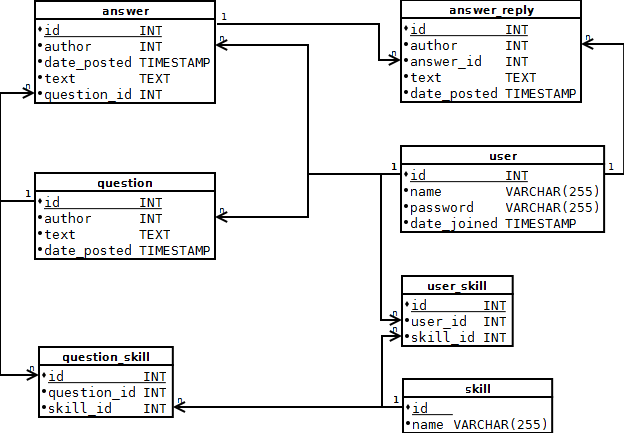
\includegraphics[width=400px]{img/erd}
	\caption{Entity relationship diagram of the database.}
	\label{figure:erd}
\end{figure}

\subsection{Remarks}

Although the relational database certainly will do the job in this case, under certain conditions NoSQL databases scale better when huge quantities of data are involved. As a result, if this app would be used by a great number of students, it is not unlikely that another design choice may outperform this one.



% REST
\section{Server}
% php (alternative google app engine)

The REST API is implemented using the codeigniter framework. Codeigniter\footnote{\url{http://ellislab.com/codeigniter}} is a \texttt{PHP} framework that relies heavily on the model-view-controller design principles. Via model classes the database can be accessed. Controllers can load model classes to pass on the data to the views. A special controller, \texttt{Api}, which extends the \texttt{REST\_Controller}\footnote{The source code can be found at \url{https://github.com/philsturgeon/codeigniter-restserver}} class, implements the REST service.

Each method listed in table \ref{table:rest_api} is then implemented in the \texttt{Api} class. Each method signature has as a suffix an underscore followed by the HTTP method name, e.g. for the method \emph{create} and HTTP method POST, this results in \emph{create\_post}. The class diagram of the backend of the application is shown in figure \ref{figure:codeigniter:classdiagram}. Figure \ref{figure:architecture:global2} summarize the application's internal structure as discussed so far.

%% class codeigniter
\begin{figure}
	\begin{center}
		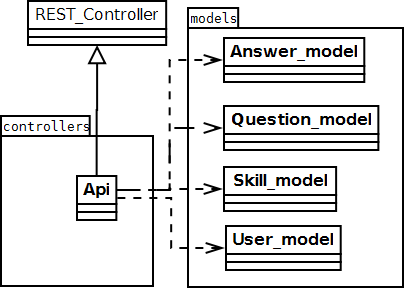
\includegraphics[width=200px]{img/codeigniter_class_diagram}
		\caption{The class diagram of the codeigniter project.}
		\label{figure:codeigniter:classdiagram}
	\end{center}
\end{figure}


%% global2
\begin{figure}
	\begin{center}
		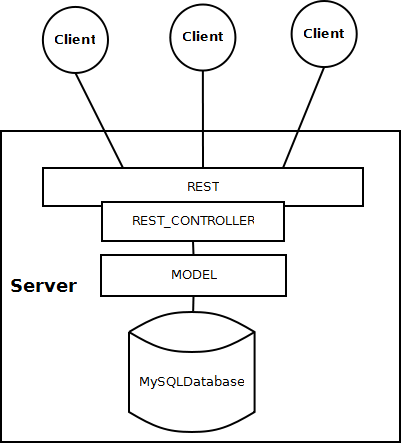
\includegraphics[width=200px]{img/architecture_global2}
		\caption{The global architecture of the application, including REST, the Codeigniter MVC design and the MySQL database.}
		\label{figure:architecture:global2}
	\end{center}
\end{figure}

Alternative libraries for REST and PHP exist, but also for other technologies, such as GAE. For example the Boomi Appengine REST Server\footnote{\url{https://code.google.com/p/appengine-rest-server/}} is a library for Google App Engine applications. Of course, this would also require a somewhat different underlying data model as mentioned earlier.

\subsection{Remarks}

When designing an API as described above, it is important to ensure that the data remains consistent. In this case, the login functionality forms a possible danger in that respect, as a user may log in from multiple apps simultaneously, and the server doesn't keep track of the number of logged in apps per user account. At the moment the session key is required to ensure that no one else log out any other user. Instead, a solution might be to create a separate table to keep track of these sessions, rather than keep a single session key entry in the user table.

If we were to create only the mobile web app, which depending on the type of application, is quite reasonable, implementing a REST API may seem like overkill. Instead a simpler design could be used to persist data. Nonetheless, when developing multiple native applications, the cost savings of creating a back-end to process parts of the data may be significant. For example, graphical operations that require a lot of computational power may be done on the device itself, while operations on the data may be done on the server.

Coming back to the point raised earlier on the performance bottleneck of a relational database. Suppose this is the case, having a well-defined API provides transparency, as the clients depend on the public interface, rather than how everything works under the hood.



\section{Clients}

Now that we have discussed the server side of the architecture, we will take a closer look at the different clients. For this project, very few code was actually written at the client side. Eventually it has become merely an experiment to test the client-server architecture, rather than an elaborate implementation of the application as described in chapter \ref{chapter:requirement_analysis}. Nonetheless, we will focus further on how the final elements of the architecture fall into place for each app.


\subsection{HTML5 mobile web application}

The \texttt{HTML5} mobile web application is basically implemented as an \texttt{HTML} web page enhanced with the jQuery mobile library\footnote{\url{http://jquerymobile.com/}}. The internal architecture consists out of JavaScript, HTML and CSS. The JavaScript code consists out of a number of libraries and source code making the connection to the back-end and controlling the view. The jQuery mobile library provides a layer on top of the original JavaScript to facilitate operations for modifying the view and the use of AJAX. A second library mirrors the REST API methods and helps to provide additional transparency when making asynchronous calls to the server. The resulting application structure is shown in figure \ref{figure:html5:architecture}.

%% architecture HTML5
\begin{figure}
	\begin{center}
		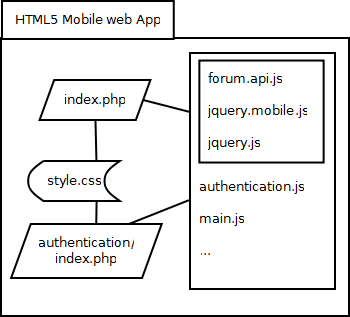
\includegraphics[width=200px]{img/html5_architecture}
		\caption{The internal structure of the HTML5 mobile web app.}
		\label{figure:html5:architecture}
	\end{center}
\end{figure}


Listing \ref{listing:html5:api} shows how the connection is made to the server in the api library. Listing \ref{listing:html5:api:use} shows how it is used in the application. An asynchronous call is made to the server. Once the result is available the anonymous function on line 5 to 13 in listing \ref{listing:html5:api:use} is executed.

\lstinputlisting[language=Java, firstline=1, lastline=16, caption={A method from the JavaScript API library to make the connection to the server.}, label={listing:html5:api}]{code/forum.api.js}

\lstinputlisting[language=Java, firstline=1, lastline=15, caption={Calling a method from the JavaScript API library.}, label={listing:html5:api:use}]{code/authentication.js}


\subsection{Android application}

The Android application follows a similar design. A seperate collection of classes provides transparent access to the REST methods of the server, as shown in figure \ref{figure:android:architecture}. Instead of passing an anonymous function as parameter, a specific listener is implemented for each asynchronous operation. Once the data is available, the notify method of the listener is called. The custom implementation of this method deals with the result from the request. This is shown in listings \ref{listing:android:api}, \ref{listing:android:listener} and \ref{listing:android:activity}. The corresponding class diagram is shown in figure \ref{figure:android:classdiagram}.

%% architecture Android
\begin{figure}
	\begin{center}
		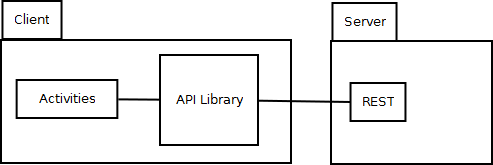
\includegraphics[width=300px]{img/android_architecture}
		\caption{The internal structure of the Android native app.}
		\label{figure:android:architecture}
	\end{center}
\end{figure}

\lstinputlisting[language=Java, firstline=6, lastline=36, caption={AnsyncTask to execute an asynchronous request to the REST server.}, label={listing:android:api}]{code/Authentication.java}

\lstinputlisting[language=Java, firstline=1, lastline=3, caption={Listener for the StartSession task.}, label={listing:android:listener}]{code/StartSessionListener.java}

\lstinputlisting[language=Java, firstline=1, lastline=15, caption={Activity that implements the StartSession listener.}, label={listing:android:activity}]{code/MainActivity.java}

%% class diagram Android
\begin{figure}
	\begin{center}
		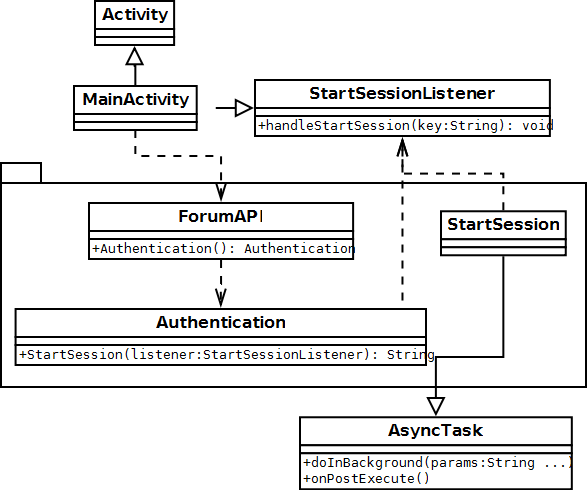
\includegraphics[width=350px]{img/android_class_diagram}
		\caption{Class diagram for the Android app.}
		\label{figure:android:classdiagram}
	\end{center}
\end{figure}


\subsection{iOS application}

Unfortunately no implementation for iOS has been completed. The global structure of the class diagram for the application would have been relatively similar to the Android application, cf. figure \ref{figure:android:architecture}, again with a separate library, which can be implemented in iOS through a static library\footnote{\url{https://developer.apple.com/library/ios/technotes/iOSStaticLibraries/Introduction.html}}, or model classes that are mapped onto the REST service's resources.

To work with REST on iOS, the RESTKit\footnote{\url{http://restkit.org/}; a recent tutorial can be found here: \url{http://www.raywenderlich.com/13097/intro-to-restkit-tutorial}} library can be used for this purpose.




\chapter{Comparison}\label{chapter:comparison}

% Mobile versus native
% iOS versus Android

\section{Web versus native mobile applications}

In \cite{Charland:2011:MAD:1941487.1941504} a table is presented of the required skill set to be able to write mobile applications for each platform. From the nine mobile technologies that were included, the market shares for Android and iOS operating systems are 68.3\% and 18.8\% respectively, clearly dominating the market \cite{Graziano:2012}. Numbers suggest that the Windows Phone will establish itself as another giant on the market, however still considerably less significant than Android or iOS. Even though this suggests development of native applications can be reduced to development for two to three technologies, the cost of developing and maintaining applications in these technologies would still create a considerable overhead. Charland et al. \cite{Charland:2011:MAD:1941487.1941504} look at mobile web technology to address this issue of heterogeneity.


\subsection{Phonegap hack}

The 'Phonegap hack' has grown from the fact that all mobile operating systems are equipped with a mobile browser, in which the native API can be called by using JavaScript. Unfortunately there are differences between the Webkit implementations of these browsers. In recent years many of these issues are being addressed through various libraries, e.g. jQuery Mobile. Also, the W3C has a device API working group that is working to bridge the gap between lower level native APIs and web technology \cite{Charland:2011:MAD:1941487.1941504}. JavaScript virtual machine technology is quickly getting more powerful, driven by competition between browsers. In the end, in \cite{Charland:2011:MAD:1941487.1941504} is stated that 'if you want to add a native capability to a browser, then you can either bridge it or recompile the browser to achieve that capability'.


\begin{quotation}
	If a browser does not support a native capability, it's not because it can't or that it won't; it just means it hasn't been done yet (Charland et al.).
\end{quotation}


\subsection{Trade-offs}

A brief list of trade-offs between web and native mobile applications:
Size of the code base - the code base for a mobile web application will be significantly smaller than the code base for two or more native applications;
Efficiency of maintenance - the cost of maintenance may be directly related to the number of versions of an application that need to be updated;
Application performance - native applications still outperform mobile web applications;
Development time;
Application objectives - related to application performance, as nice looking visuals do not fulfill business requirements, but may require significantly more processing power;
GUI guidelines: creating only one application for different platforms, may require a lot of conditional statements to provide user interface code that is conform with the guidelines for each seperate platform;

% CONCLUSION
\chapter{Conclusion}\label{chapter:conclusion}




%%%%%%%%%%%%%%%%%%%%%%%%%%%%%%%%%%%%%%%%%%%%%%%%%%%%%%%%%%%%%
%% BIBLIOGRAPHY AND OTHER LISTS
%%%%%%%%%%%%%%%%%%%%%%%%%%%%%%%%%%%%%%%%%%%%%%%%%%%%%%%%%%%%%
%% A small distance to the other stuff in the table of contents (toc)
\addtocontents{toc}{\protect\vspace*{\baselineskip}}

%% The Bibliography
\addcontentsline{toc}{chapter}{References} %'Bibliography' into toc
%\bibliographystyle{alpha} %Style of Bibliography: plain / apalike / amsalpha / ...
\bibliographystyle{abbrv}
\bibliography{bib/references} %You need a file 'literature.bib' for this.


%% The List of Figures
\clearpage
\addcontentsline{toc}{chapter}{List of Figures}
\listoffigures

%% The List of Tables
\clearpage
\addcontentsline{toc}{chapter}{List of Tables}
\listoftables


%%%%%%%%%%%%%%%%%%%%%%%%%%%%%%%%%%%%%%%%%%%%%%%%%%%%%%%%%%%%%
%% APPENDICES
%%%%%%%%%%%%%%%%%%%%%%%%%%%%%%%%%%%%%%%%%%%%%%%%%%%%%%%%%%%%%
%\appendix

% how to set up the codeigniter environment and REST API
%\chapter{Codeigniter and REST API Setup}



% how to use the api with the different technologies
%\chapter{REST API}\label{app:rest}

\begin{table}
	\caption{REST API}\label{table:rest_api}
	
	\begin{center}
		\begin{tabular}{p{70px} | p{70px} | p{210px}}
				\hline
				\hline
				\textbf{Resource} 		& \textbf{Method}					&	\textbf{Description} 	\\
				\hline
				\hline
				\texttt{ANSWER}				& 												&	\\
				\hline
															& \emph{create}						& Create a new answer. \\
															& \emph{get\_question}		& Get the question this answer was posted on. \\
															%& \emph{search}						& Search an answer.	\\
				\hline
				\texttt{AUTHENTICATION}		& 												&	\\
				\hline
															& \emph{endsession}				& Create a new answer. \\
															& \emph{startsession}			& Get the question this answer was posted on. \\
				\hline
				\texttt{QUESTION}			& 												& \\
				\hline
															& \emph{create}						& Post a new question. \\
															& \emph{get\_answers}			& Get the answers for a question. \\
															& \emph{get\_info}				& Get information on a question. \\
															& \emph{get\_skills}			& Get the skills related to this question. \\
															& \emph{remove}						& Delete a question. \\
															%& \emph{search}						& Search questions, given a number of search parameters. \\
				\hline
				\texttt{SKILL}				& 												& \\
				\hline
															& \emph{create}						& Create a new skill and add it to the database. \\
															& \emph{get\_questions}		& Get questions related to a given skill. \\
															%& \emph{search}						& Search skills. \\
				\hline
				\texttt{USER}					&	\\
				\hline
															& \emph{get\_answers}			& Get the answers submitted by a user. \\
															& \emph{get\_questions}		& Get questions submitted by a user. \\
															& \emph{get\_info}				&	Retrieve profile information about a user.	\\
															& \emph{get\_skills}			& Get the skills of a user. \\
															& \emph{register}					&	Register a new user account. \\
															& \emph{search}						&	Search a user given certain parameters. \\
															& \emph{unregister}				&	Delete a user account. \\
															& \emph{update\_info}			& Update profile information about a user. \\
															%& \emph{getContacts}	  	& \\
															%& \emph{}									& \\
				\hline
				\hline
		\end{tabular}
	\end{center}
	
\end{table}



% stats
%\chapter{Statistics}




%%%%%%%%%%%%%%%%%%%%%%%%END DOCUMENT%%%%%%%%%%%%%%%%%%%%%%%%%
\end{document}

